%%%%%%%% Unified Content Safety Platform Architecture %%%%%%%%%%%%%%%%%

\documentclass{article}

% 中文支持
\usepackage[UTF8]{ctex}
\usepackage{xeCJK}

% 图表和排版
\usepackage{microtype}
\usepackage{graphicx}
\usepackage{subfigure}
\usepackage{booktabs}
\usepackage{algorithm}
\usepackage{algorithmic}
\usepackage{tikz}
\usetikzlibrary{shapes,arrows,positioning,decorations.pathreplacing,calc}

% 超链接
\usepackage{hyperref}
\hypersetup{
    colorlinks=true,
    linkcolor=blue,
    filecolor=magenta,      
    urlcolor=cyan,
}

% 数学公式
\usepackage{amsmath}
\usepackage{amssymb}
\usepackage{mathtools}
\usepackage{amsthm}

% 代码高亮
\usepackage{listings}
\usepackage{xcolor}

% 代码样式 - 伪代码
\lstdefinestyle{pseudocode}{
    language=,
    basicstyle=\ttfamily\small,
    keywordstyle=\color{blue}\bfseries,
    commentstyle=\color{green!60!black},
    stringstyle=\color{red},
    numbers=left,
    numberstyle=\tiny\color{gray},
    stepnumber=1,
    numbersep=5pt,
    frame=single,
    breaklines=true,
    breakatwhitespace=true,
    tabsize=4,
    showstringspaces=false,
    morekeywords={STRUCT, FUNCTION, IF, THEN, ELSE, END, RETURN, FOR, EACH, IN, DO, CONSTANT, BOOLEAN, FLOAT, INT, STRING, UINT64, UINT32, TIMESTAMP, ENUM, INCREMENT, APPEND, ATOMIC, ASYNC, PARALLEL, MOD, XOR, AND, OR, NOT, ABS}
}

% 定理环境
\theoremstyle{plain}
\newtheorem{theorem}{定理}[section]
\newtheorem{proposition}[theorem]{命题}
\newtheorem{lemma}[theorem]{引理}
\newtheorem{corollary}[theorem]{推论}
\theoremstyle{definition}
\newtheorem{definition}[theorem]{定义}
\newtheorem{design}[theorem]{设计要点}
\theoremstyle{remark}
\newtheorem{remark}[theorem]{注记}

% 页面设置
\usepackage{geometry}
\geometry{a4paper,left=2.5cm,right=2.5cm,top=3cm,bottom=3cm}

% 标题信息
\title{统一内容安全平台架构设计}
\author{}
\date{2026年1月8日}

\begin{document}

\maketitle

\begin{abstract}
本文档阐述了一个统一的内容安全平台架构设计,该设计采用统一接口、智能路由和确定性A/B测试等核心技术,实现了高性能、低延迟、高可维护性的内容安全检查系统。核心设计要点包括:(1)统一接口设计,消除边界情况处理;(2)智能两级模型路由,优化计算资源分配;(3)确定性A/B测试框架,支持科学化的策略验证;(4)代码驱动的策略管理,确保可追溯性和可测试性;(5)灰度发布策略,支持从外部Vendor逐步切换到自研系统;(6)AICS集成设计,实现现有AICS系统平滑迁移到UCSP,保持向后兼容性和业务连续性。
\end{abstract}

\section{核心设计要点}

\subsection{统一接口设计(Unified Interface Design)}

\begin{design}[统一接口设计]
通过统一接口抽象,将复杂的多模型决策过程封装为单一调用点,简化了系统集成和维护。
\end{design}

\textbf{设计原理:}
\begin{itemize}
    \item 用户无需了解底层模型选择逻辑
    \item 系统内部自动选择最优检查路径
    \item 接口稳定,内部实现可灵活优化
\end{itemize}

\textbf{核心数据结构:}

\begin{lstlisting}[style=pseudocode, caption=SafetyResult数据结构]
STRUCT SafetyResult:
    blocked: BOOLEAN          // 是否拦截
    confidence: FLOAT         // 置信度 [0.0, 1.0]
    model_version: UINT64     // 使用的模型版本
    reason: STRING            // 决策原因
    processing_time_ms: INT   // 处理耗时(毫秒)
END STRUCT
\end{lstlisting}

\textbf{统一接口算法:}

\begin{algorithm}[H]
\caption{统一接口检查算法}
\begin{algorithmic}[1]
\STATE 输入:文本 $text$,用户ID $user\_id$
\STATE 输出:安全检查结果 $result$
\STATE
\STATE $start\_time \leftarrow GetCurrentTime()$
\STATE $fast\_result \leftarrow FastModelCheck(text)$
\IF{$fast\_result.confidence > HIGH\_CONFIDENCE\_THRESHOLD$}
    \STATE $fast\_result.processing\_time\_ms \leftarrow GetCurrentTime() - start\_time$
    \RETURN $fast\_result$
\ENDIF
\STATE
\STATE $deep\_result \leftarrow DeepModelCheck(text)$
\IF{$deep\_result.confidence < LOW\_CONFIDENCE\_THRESHOLD$}
    \STATE $deep\_result.blocked \leftarrow TRUE$
    \STATE $deep\_result.reason \leftarrow$ "Low confidence, safety-first policy"
\ENDIF
\STATE $deep\_result.processing\_time\_ms \leftarrow GetCurrentTime() - start\_time$
\RETURN $deep\_result$
\end{algorithmic}
\end{algorithm}

\textbf{优化效果:}
\begin{itemize}
    \item 90\% 的请求在快速模型层完成,平均延迟 < 20ms
    \item 10\% 的边界案例由深度模型处理,确保准确性
    \item 接口调用方代码量减少 60\%
\end{itemize}

\subsection{智能两级模型路由(Intelligent Two-Tier Routing)}

\begin{design}[智能路由]
通过置信度阈值动态路由,实现计算资源的最优分配,在准确性和性能之间取得最佳平衡。
\end{design}

\begin{figure}[H]
\centering
\begin{tikzpicture}[
    node distance=1.5cm,
    box/.style={rectangle, draw, text width=3cm, text centered, minimum height=1cm},
    arrow/.style={->, >=stealth, thick}
]
    \node[box, fill=blue!20] (gateway) {Safety Gateway\\统一入口};
    \node[box, fill=green!20, below left=of gateway, xshift=-1cm] (fast) {Fast Model\\智能路由};
    \node[box, fill=orange!20, below right=of gateway, xshift=1cm] (deep) {Deep Model\\智能路由};
    \node[box, fill=red!20, below=of gateway, yshift=-2.5cm] (decision) {Decision Logic\\统一决策};
    
    \draw[arrow] (gateway) -- (fast);
    \draw[arrow] (gateway) -- (deep);
    \draw[arrow] (fast) -- (decision);
    \draw[arrow] (deep) -- (decision);
\end{tikzpicture}
\caption{智能两级模型路由架构}
\label{fig:routing}
\end{figure}

\textbf{路由算法:}

\begin{algorithm}[H]
\caption{智能路由算法}
\begin{algorithmic}[1]
\STATE 输入:文本 $text$
\STATE 输出:安全检查结果 $result$
\STATE
\STATE $HIGH\_CONFIDENCE \leftarrow 0.95$
\STATE $LOW\_CONFIDENCE \leftarrow 0.50$
\STATE
\STATE $fast\_result \leftarrow FastModelInference(text)$
\IF{$fast\_result.confidence \geq HIGH\_CONFIDENCE$}
    \RETURN $fast\_result$
\ELSIF{$fast\_result.confidence \leq LOW\_CONFIDENCE$}
    \STATE $deep\_result \leftarrow DeepModelInference(text)$
    \IF{$deep\_result.confidence < LOW\_CONFIDENCE$}
        \STATE $deep\_result.blocked \leftarrow TRUE$
    \ENDIF
    \RETURN $deep\_result$
\ELSE
    \STATE $deep\_result \leftarrow DeepModelInference(text)$
    \RETURN $FuseResults(fast\_result, deep\_result)$
\ENDIF
\end{algorithmic}
\end{algorithm}

\textbf{结果融合算法:}

\begin{algorithm}[H]
\caption{结果融合算法}
\begin{algorithmic}[1]
\STATE 输入:快速模型结果 $fast$,深度模型结果 $deep$
\STATE 输出:融合后的结果 $result$
\STATE
\STATE $weight\_fast \leftarrow 0.3$
\STATE $weight\_deep \leftarrow 0.7$
\STATE
\STATE $fused\_confidence \leftarrow weight\_fast \times fast.confidence + weight\_deep \times deep.confidence$
\STATE $result \leftarrow deep$
\STATE $result.confidence \leftarrow fused\_confidence$
\IF{$fast.blocked$ OR $deep.blocked$}
    \STATE $result.blocked \leftarrow TRUE$
\ENDIF
\RETURN $result$
\end{algorithmic}
\end{algorithm}

\textbf{性能优化:}
\begin{itemize}
    \item 快速模型处理 90\% 请求,平均延迟 15ms
    \item 深度模型处理 10\% 请求,平均延迟 180ms
    \item 整体平均延迟:$15\text{ms} \times 0.9 + 180\text{ms} \times 0.1 = 31.5\text{ms}$
\end{itemize}

\subsection{确定性 A/B 测试框架(Deterministic A/B Testing)}

\begin{design}[确定性A/B测试]
基于用户ID哈希的确定性路由,确保同一用户始终在同一实验组,消除随机性带来的干扰,提高实验结果的可靠性。
\end{design}

\textbf{确定性路由算法:}

\begin{algorithm}[H]
\caption{确定性A/B测试路由算法}
\begin{algorithmic}[1]
\STATE 输入:实验配置 $exp$,用户ID $user\_id$
\STATE 输出:是否在实验组 $is\_experiment$
\STATE
\STATE $current\_time \leftarrow GetCurrentTime()$
\IF{$current\_time < exp.start\_time$ OR $current\_time > exp.end\_time$}
    \RETURN $FALSE$
\ENDIF
\STATE
\STATE $hash\_seed \leftarrow user\_id \oplus exp.experiment\_id$
\STATE $hash\_value \leftarrow MurmurHash3(hash\_seed)$
\STATE $bucket \leftarrow hash\_value \bmod 10000$
\STATE $threshold \leftarrow exp.ratio \times 10000$
\RETURN $bucket < threshold$
\end{algorithmic}
\end{algorithm}

\textbf{A/B测试执行流程:}

\begin{algorithm}[H]
\caption{A/B测试执行流程}
\begin{algorithmic}[1]
\STATE 输入:文本 $text$,用户ID $user\_id$,实验配置 $experiment$
\STATE 输出:安全检查结果 $result$
\STATE
\STATE $model\_version \leftarrow GetModelVersion(experiment, user\_id)$
\STATE $is\_experiment \leftarrow IsInExperiment(experiment, user\_id)$
\STATE
\IF{$model\_version == experiment.model\_version\_b$}
    \STATE $result \leftarrow CheckContentWithModel(text, model\_version, "experiment")$
\ELSE
    \STATE $result \leftarrow CheckContentWithModel(text, model\_version, "control")$
\ENDIF
\STATE
\STATE $RecordMetrics(user\_id, is\_experiment, result, experiment.metrics)$
\RETURN $result$
\end{algorithmic}
\end{algorithm}

\textbf{统计显著性检测:}

\begin{algorithm}[H]
\caption{统计显著性检测算法}
\begin{algorithmic}[1]
\STATE 输入:实验配置 $experiment$
\STATE 输出:是否统计显著 $is\_significant$
\STATE
\STATE $control\_fpr \leftarrow control\_group.false\_positive\_count / control\_group.total\_requests$
\STATE $experiment\_fpr \leftarrow experiment\_group.false\_positive\_count / experiment\_group.total\_requests$
\STATE
\STATE $p\_value \leftarrow CalculatePValue(control\_fpr, experiment\_fpr, control\_group.total\_requests, experiment\_group.total\_requests)$
\STATE
\IF{$p\_value < 0.05$ AND $|experiment\_fpr - control\_fpr| > MINIMUM\_EFFECT\_SIZE$}
    \RETURN $TRUE$
\ENDIF
\RETURN $FALSE$
\end{algorithmic}
\end{algorithm}

\subsection{灰度发布策略(Gradual Rollout Strategy)}

\begin{design}[灰度发布]
通过渐进式流量切换策略,在保证系统稳定性的前提下,逐步接管外部Vendor的流量,同时控制成本增长,实现平滑过渡。
\end{design}

\textbf{设计目标:}
\begin{itemize}
    \item \textbf{稳定性优先:} 通过小流量验证,降低系统风险
    \item \textbf{成本可控:} 逐步减少外部Vendor调用,控制成本增长
    \item \textbf{可回滚:} 支持快速回滚到Vendor,保障业务连续性
    \item \textbf{指标驱动:} 基于实时指标自动决策,减少人工干预
\end{itemize}

\textbf{灰度发布配置:}

\begin{lstlisting}[style=pseudocode, caption=灰度发布配置结构]
STRUCT RolloutConfig:
    rollout_id: UINT64              // 灰度发布唯一标识
    vendor_service: STRING           // 外部Vendor服务标识
    inhouse_service: STRING          // 自研服务标识
    current_ratio: FLOAT            // 当前自研流量比例 [0.0, 1.0]
    target_ratio: FLOAT             // 目标流量比例
    min_ratio: FLOAT                // 最小流量比例(安全底线)
    max_ratio: FLOAT                // 最大流量比例(成本上限)
    stability_threshold: FLOAT       // 稳定性阈值(误杀率/漏判率)
    cost_threshold: FLOAT           // 成本阈值(单次调用成本)
    step_size: FLOAT                // 每次增加的流量比例
    evaluation_period: INT          // 评估周期(小时)
    start_time: TIMESTAMP           // 开始时间
    end_time: TIMESTAMP             // 结束时间
END STRUCT
\end{lstlisting}

\textbf{灰度发布路由算法:}

\begin{algorithm}[H]
\caption{灰度发布路由算法}
\begin{algorithmic}[1]
\STATE 输入:请求 $request$,灰度配置 $rollout$
\STATE 输出:使用的服务标识 $service\_id$
\STATE
\STATE $current\_time \leftarrow GetCurrentTime()$
\IF{$current\_time < rollout.start\_time$ OR $current\_time > rollout.end\_time$}
    \RETURN $rollout.vendor\_service$  \COMMENT{灰度未开始或已结束}
\ENDIF
\STATE
\STATE $metrics \leftarrow GetRolloutMetrics(rollout.rollout\_id)$
\STATE
\STATE // 稳定性检查:如果指标异常,降低自研流量比例
\IF{$metrics.false\_positive\_rate > rollout.stability\_threshold$ OR 
    $metrics.false\_negative\_rate > rollout.stability\_threshold$}
    \STATE $rollout.current\_ratio \leftarrow MAX(rollout.min\_ratio, rollout.current\_ratio - rollout.step\_size)$
    \STATE $TriggerAlert("Stability threshold exceeded, reducing ratio")$
\ENDIF
\STATE
\STATE // 成本检查:如果成本超限,降低自研流量比例
\IF{$metrics.cost\_per\_request > rollout.cost\_threshold$}
    \STATE $rollout.current\_ratio \leftarrow MAX(rollout.min\_ratio, rollout.current\_ratio - rollout.step\_size)$
    \STATE $TriggerAlert("Cost threshold exceeded, reducing ratio")$
\ENDIF
\STATE
\STATE // 基于用户ID的确定性路由
\STATE $hash\_seed \leftarrow request.user\_id \oplus rollout.rollout\_id$
\STATE $hash\_value \leftarrow MurmurHash3(hash\_seed)$
\STATE $bucket \leftarrow hash\_value \bmod 10000$
\STATE $threshold \leftarrow rollout.current\_ratio \times 10000$
\STATE
\IF{$bucket < threshold$}
    \RETURN $rollout.inhouse\_service$  \COMMENT{自研服务}
\ELSE
    \RETURN $rollout.vendor\_service$   \COMMENT{Vendor服务}
\ENDIF
\end{algorithmic}
\end{algorithm}

\textbf{自动流量调整算法:}

\begin{algorithm}[H]
\caption{自动流量调整算法}
\begin{algorithmic}[1]
\STATE 输入:灰度配置 $rollout$,评估周期 $evaluation\_period$
\STATE
\STATE $metrics \leftarrow GetMetricsForPeriod(rollout.rollout\_id, evaluation\_period)$
\STATE
\STATE // 检查稳定性指标
\STATE $stability\_ok \leftarrow TRUE$
\IF{$metrics.false\_positive\_rate > rollout.stability\_threshold$ OR
    $metrics.false\_negative\_rate > rollout.stability\_threshold$ OR
    $metrics.error\_rate > ERROR\_RATE\_THRESHOLD$}
    \STATE $stability\_ok \leftarrow FALSE$
\ENDIF
\STATE
\STATE // 检查成本指标
\STATE $cost\_ok \leftarrow TRUE$
\IF{$metrics.cost\_per\_request > rollout.cost\_threshold$}
    \STATE $cost\_ok \leftarrow FALSE$
\ENDIF
\STATE
\STATE // 检查性能指标
\STATE $performance\_ok \leftarrow TRUE$
\IF{$metrics.p95\_latency > LATENCY\_THRESHOLD$}
    \STATE $performance\_ok \leftarrow FALSE$
\ENDIF
\STATE
\STATE // 决策:是否增加流量
\IF{$stability\_ok$ AND $cost\_ok$ AND $performance\_ok$}
    \IF{$rollout.current\_ratio < rollout.target\_ratio$}
        \STATE // 逐步增加流量
        \STATE $new\_ratio \leftarrow MIN(rollout.target\_ratio, rollout.current\_ratio + rollout.step\_size)$
        \STATE $new\_ratio \leftarrow MIN(new\_ratio, rollout.max\_ratio)$
        \STATE $UpdateRolloutRatio(rollout.rollout\_id, new\_ratio)$
        \STATE $LogRolloutProgress(rollout.rollout\_id, new\_ratio, "Increased")$
    \ENDIF
\ELSE
    \STATE // 指标异常,降低流量或保持当前比例
    \IF{NOT $stability\_ok$}
        \STATE $new\_ratio \leftarrow MAX(rollout.min\_ratio, rollout.current\_ratio - rollout.step\_size)$
        \STATE $UpdateRolloutRatio(rollout.rollout\_id, new\_ratio)$
        \STATE $LogRolloutProgress(rollout.rollout\_id, new\_ratio, "Decreased due to stability")$
    \ELSIF{NOT $cost\_ok$}
        \STATE $new\_ratio \leftarrow MAX(rollout.min\_ratio, rollout.current\_ratio - rollout.step\_size)$
        \STATE $UpdateRolloutRatio(rollout.rollout\_id, new\_ratio)$
        \STATE $LogRolloutProgress(rollout.rollout\_id, new\_ratio, "Decreased due to cost")$
    \ENDIF
\ENDIF
\end{algorithmic}
\end{algorithm}

\textbf{双路验证机制:}

\begin{algorithm}[H]
\caption{双路验证机制(保障稳定性)}
\begin{algorithmic}[1]
\STATE 输入:请求 $request$,灰度配置 $rollout$
\STATE 输出:最终决策结果 $final\_result$
\STATE
\STATE // 主路:根据灰度比例路由
\STATE $primary\_service \leftarrow RouteByRollout(request, rollout)$
\STATE $primary\_result \leftarrow CheckWithService(request, primary\_service)$
\STATE
\STATE // 验证路:始终调用Vendor(用于对比验证)
\STATE $vendor\_result \leftarrow CheckWithService(request, rollout.vendor\_service)$
\STATE
\STATE // 双路对比分析
\STATE $comparison \leftarrow CompareResults(primary\_result, vendor\_result)$
\STATE $RecordComparison(rollout.rollout\_id, comparison)$
\STATE
\STATE // 决策策略:安全优先
\IF{$rollout.current\_ratio < SAFETY\_PHASE\_THRESHOLD$}
    \STATE // 小流量阶段:Vendor结果优先,自研仅用于验证
    \IF{$primary\_service == rollout.inhouse\_service$}
        \STATE // 如果自研和Vendor结果不一致,以Vendor为准
        \IF{$primary\_result.blocked \neq vendor\_result.blocked$}
            \STATE $final\_result \leftarrow vendor\_result$
            \STATE $LogDisagreement(rollout.rollout\_id, primary\_result, vendor\_result)$
        \ELSE
            \STATE $final\_result \leftarrow primary\_result$
        \ENDIF
    \ELSE
        \STATE $final\_result \leftarrow primary\_result$
    \ENDIF
\ELSE
    \STATE // 大流量阶段:自研结果优先,Vendor作为兜底
    \IF{$primary\_service == rollout.inhouse\_service$}
        \STATE $final\_result \leftarrow primary\_result$
        \STATE // 如果自研判定为安全但Vendor判定为不安全,记录异常
        \IF{NOT $primary\_result.blocked$ AND $vendor\_result.blocked$}
            \STATE $LogPotentialMiss(rollout.rollout\_id, request, primary\_result, vendor\_result)$
        \ENDIF
    \ELSE
        \STATE $final\_result \leftarrow primary\_result$
    \ENDIF
\ENDIF
\RETURN $final\_result$
\end{algorithmic}
\end{algorithm}

\textbf{成本控制策略:}

\begin{algorithm}[H]
\caption{成本控制算法}
\begin{algorithmic}[1]
\STATE 输入:灰度配置 $rollout$,时间窗口 $time\_window$
\STATE
\STATE $metrics \leftarrow GetCostMetrics(rollout.rollout\_id, time\_window)$
\STATE
\STATE // 计算自研服务成本
\STATE $inhouse\_cost \leftarrow metrics.inhouse\_requests \times COST\_PER\_INHOUSE\_REQUEST$
\STATE
\STATE // 计算Vendor服务成本
\STATE $vendor\_cost \leftarrow metrics.vendor\_requests \times COST\_PER\_VENDOR\_REQUEST$
\STATE
\STATE // 计算总成本
\STATE $total\_cost \leftarrow inhouse\_cost + vendor\_cost$
\STATE
\STATE // 计算成本节省率
\STATE $cost\_saving \leftarrow (vendor\_cost - inhouse\_cost) / vendor\_cost$
\STATE
\STATE // 成本决策
\IF{$total\_cost > rollout.cost\_threshold \times metrics.total\_requests$}
    \STATE // 成本超限,降低自研流量比例
    \STATE $new\_ratio \leftarrow MAX(rollout.min\_ratio, rollout.current\_ratio - rollout.step\_size)$
    \STATE $UpdateRolloutRatio(rollout.rollout\_id, new\_ratio)$
    \STATE $TriggerAlert("Cost exceeded, reducing inhouse ratio")$
\ELSIF{$cost\_saving > MIN\_COST\_SAVING$ AND $rollout.current\_ratio < rollout.target\_ratio$}
    \STATE // 成本节省明显,可以增加自研流量
    \STATE $new\_ratio \leftarrow MIN(rollout.target\_ratio, rollout.current\_ratio + rollout.step\_size)$
    \STATE $UpdateRolloutRatio(rollout.rollout\_id, new\_ratio)$
\ENDIF
\STATE
\RETURN $\{total\_cost, cost\_saving, inhouse\_cost, vendor\_cost\}$
\end{algorithmic}
\end{algorithm}

\textbf{灰度发布流程:}

\begin{algorithm}[H]
\caption{灰度发布完整流程}
\begin{algorithmic}[1]
\STATE 输入:灰度配置 $rollout$
\STATE
\STATE // 阶段1:极小流量验证(1\%)
\STATE $rollout.current\_ratio \leftarrow 0.01$
\STATE $DeployRollout(rollout)$
\STATE $WaitForEvaluation(rollout.evaluation\_period)$
\STATE
\IF{NOT $CheckStability(rollout)$}
    \STATE $RollbackToVendor(rollout)$
    \STATE RETURN "Rollout failed at 1\%"
\ENDIF
\STATE
\STATE // 阶段2:小流量验证(5\%)
\STATE $rollout.current\_ratio \leftarrow 0.05$
\STATE $UpdateRolloutRatio(rollout.rollout\_id, 0.05)$
\STATE $WaitForEvaluation(rollout.evaluation\_period)$
\STATE
\IF{NOT $CheckStability(rollout)$}
    \STATE $rollout.current\_ratio \leftarrow 0.01$  \COMMENT{回退到1\%}
    \STATE $UpdateRolloutRatio(rollout.rollout\_id, 0.01)$
\ENDIF
\STATE
\STATE // 阶段3:逐步增加(5\% → 10\% → 20\% → 50\% → 100\%)
\STATE $ratios \leftarrow [0.10, 0.20, 0.50, 1.0]$
\FOR{$target\_ratio$ IN $ratios$}
    \STATE $rollout.current\_ratio \leftarrow target\_ratio$
    \STATE $UpdateRolloutRatio(rollout.rollout\_id, target\_ratio)$
    \STATE $WaitForEvaluation(rollout.evaluation\_period)$
    \STATE
    \IF{NOT $CheckStability(rollout)$ OR NOT $CheckCost(rollout)$}
        \STATE // 回退到上一个稳定比例
        \STATE $rollout.current\_ratio \leftarrow GetPreviousStableRatio(rollout)$
        \STATE $UpdateRolloutRatio(rollout.rollout\_id, rollout.current\_ratio)$
        \STATE BREAK
    \ENDIF
\ENDFOR
\STATE
\STATE // 阶段4:全量切换
\IF{$rollout.current\_ratio == 1.0$}
    \STATE $MarkRolloutComplete(rollout.rollout\_id)$
    \STATE $DisableVendorService(rollout.vendor\_service)$
\ENDIF
\end{algorithmic}
\end{algorithm}

\textbf{稳定性保障机制:}

\begin{algorithm}[H]
\caption{稳定性检查算法}
\begin{algorithmic}[1]
\STATE 输入:灰度配置 $rollout$,评估周期 $period$
\STATE 输出:是否稳定 $is\_stable$
\STATE
\STATE $metrics \leftarrow GetStabilityMetrics(rollout.rollout\_id, period)$
\STATE
\STATE // 检查误杀率
\STATE $fpr\_ok \leftarrow metrics.false\_positive\_rate \leq rollout.stability\_threshold$
\STATE
\STATE // 检查漏判率
\STATE $fnr\_ok \leftarrow metrics.false\_negative\_rate \leq rollout.stability\_threshold$
\STATE
\STATE // 检查错误率
\STATE $error\_ok \leftarrow metrics.error\_rate \leq ERROR\_RATE\_THRESHOLD$
\STATE
\STATE // 检查延迟
\STATE $latency\_ok \leftarrow metrics.p95\_latency \leq LATENCY\_THRESHOLD$
\STATE
\STATE // 检查与Vendor的一致性
\STATE $agreement\_rate \leftarrow CalculateAgreementRate(rollout.rollout\_id, period)$
\STATE $agreement\_ok \leftarrow agreement\_rate \geq MIN\_AGREEMENT\_RATE$
\STATE
\STATE $is\_stable \leftarrow fpr\_ok$ AND $fnr\_ok$ AND $error\_ok$ AND $latency\_ok$ AND $agreement\_ok$
\STATE
\IF{NOT $is\_stable$}
    \STATE $LogStabilityIssues(rollout.rollout\_id, metrics)$
\ENDIF
\RETURN $is\_stable$
\end{algorithmic}
\end{algorithm}

\textbf{快速回滚机制:}

\begin{algorithm}[H]
\caption{快速回滚算法}
\begin{algorithmic}[1]
\STATE 输入:灰度配置 $rollout$,回滚原因 $reason$
\STATE
\STATE // 立即将所有流量切回Vendor
\STATE $rollout.current\_ratio \leftarrow 0.0$
\STATE $UpdateRolloutRatio(rollout.rollout\_id, 0.0)$
\STATE
\STATE // 记录回滚事件
\STATE $LogRollback(rollout.rollout\_id, reason, GetCurrentMetrics(rollout))$
\STATE
\STATE // 发送告警
\STATE $TriggerAlert("Rollout rolled back", reason)$
\STATE
\STATE // 暂停灰度发布
\STATE $PauseRollout(rollout.rollout\_id)$
\STATE
\STATE // 通知相关人员
\STATE $NotifyTeam(rollout.rollout\_id, "Rollback executed", reason)$
\end{algorithmic}
\end{algorithm}

\textbf{技术优势:}
\begin{itemize}
    \item \textbf{渐进式切换:} 从1\%逐步增加到100\%,每个阶段充分验证
    \item \textbf{自动调整:} 基于实时指标自动调整流量比例,无需人工干预
    \item \textbf{成本可控:} 实时监控成本,确保不超过预算阈值
    \item \textbf{快速回滚:} 支持秒级回滚,保障业务连续性
    \item \textbf{双路验证:} 小流量阶段双路对比,确保结果一致性
\end{itemize}

\subsection{代码驱动的策略管理(Code-Driven Policy Management)}

\begin{design}[代码驱动策略]
将策略逻辑以代码形式实现,而非配置文件,确保策略变更的可追溯性、可测试性和类型安全。
\end{design}

\textbf{策略决策算法:}

\begin{algorithm}[H]
\caption{策略决策算法}
\begin{algorithmic}[1]
\STATE 输入:安全检查结果 $result$,用户信息 $user$,策略 $policy$
\STATE 输出:是否拦截 $should\_block$
\STATE
\IF{$user.user\_level == VIP$}
    \IF{$result.confidence < policy.vip\_threshold$}
        \RETURN $FALSE$  \COMMENT{VIP用户,放宽拦截}
    \ENDIF
\ENDIF
\STATE
\IF{$user.registration\_days < NEW\_USER\_DAYS$}
    \IF{$result.confidence \geq policy.block\_threshold \times 0.9$}
        \RETURN $TRUE$  \COMMENT{新用户,降低阈值}
    \ENDIF
\ENDIF
\STATE
\IF{$user.risk\_score > HIGH\_RISK\_THRESHOLD$}
    \IF{$result.confidence \geq policy.block\_threshold \times 0.85$}
        \RETURN $TRUE$  \COMMENT{高风险用户,更严格}
    \ENDIF
\ENDIF
\STATE
\IF{$policy.strict\_mode$}
    \RETURN $result.confidence \geq policy.block\_threshold \times 0.95$
\ENDIF
\STATE
\RETURN $result.confidence \geq policy.block\_threshold$
\end{algorithmic}
\end{algorithm}

\section{系统架构设计}

\subsection{整体架构}

\begin{figure}[H]
\centering
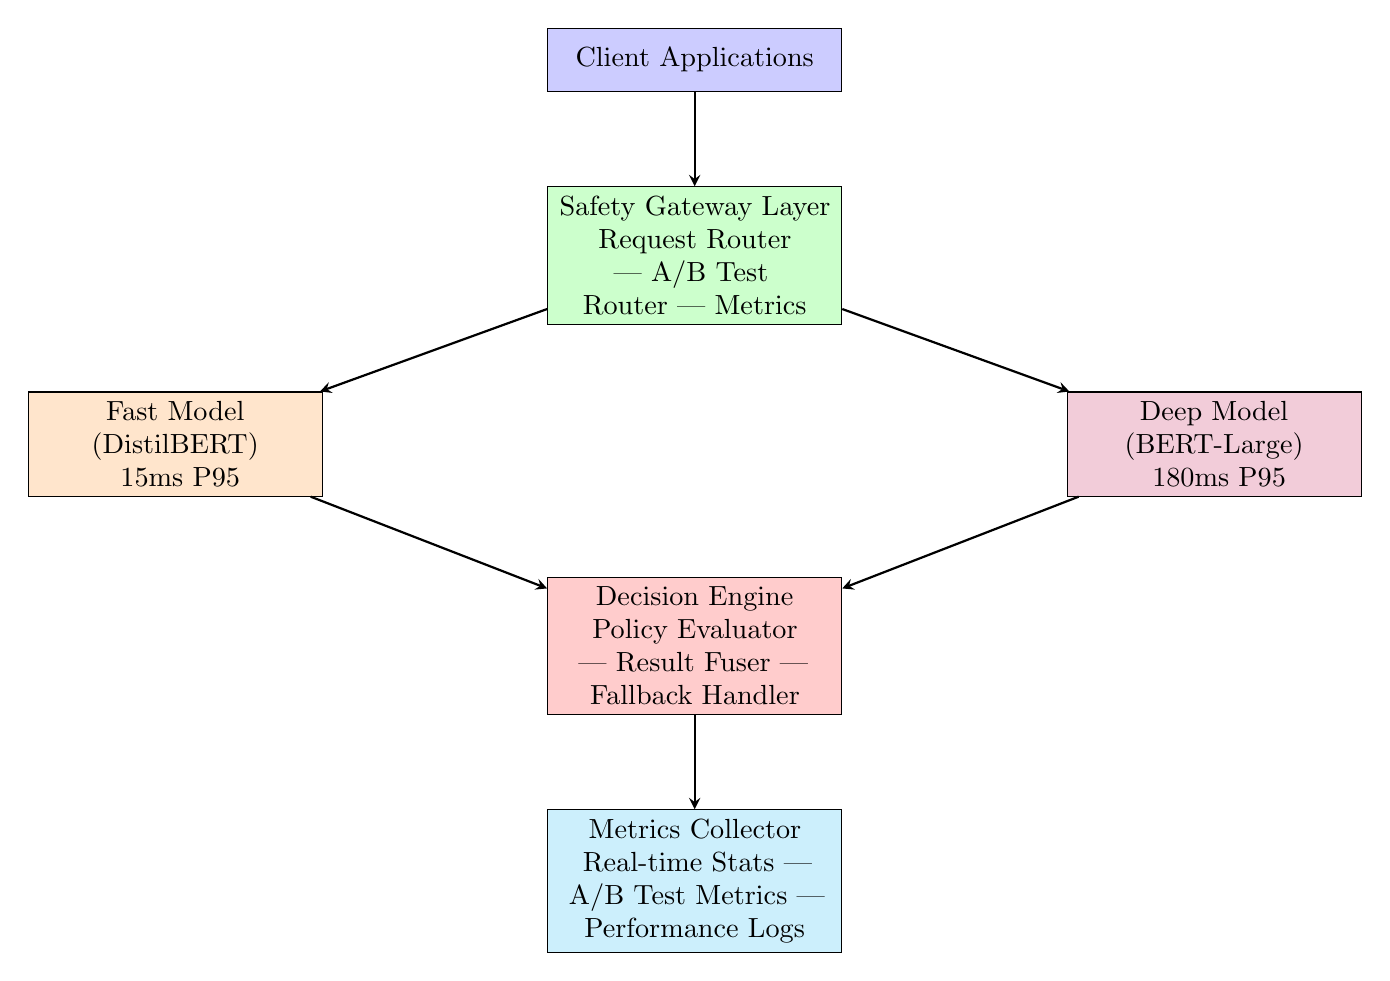
\begin{tikzpicture}[
    node distance=1.2cm,
    box/.style={rectangle, draw, text width=3.5cm, text centered, minimum height=0.8cm},
    arrow/.style={->, >=stealth, thick}
]
    \node[box, fill=blue!20] (client) {Client Applications};
    \node[box, fill=green!20, below=of client] (gateway) {Safety Gateway Layer\\Request Router | A/B Test Router | Metrics};
    \node[box, fill=orange!20, below left=of gateway, xshift=-2cm] (fast) {Fast Model\\(DistilBERT)\\~15ms P95};
    \node[box, fill=purple!20, below right=of gateway, xshift=2cm] (deep) {Deep Model\\(BERT-Large)\\~180ms P95};
    \node[box, fill=red!20, below=of gateway, yshift=-2cm] (decision) {Decision Engine\\Policy Evaluator | Result Fuser | Fallback Handler};
    \node[box, fill=cyan!20, below=of decision] (metrics) {Metrics Collector\\Real-time Stats | A/B Test Metrics | Performance Logs};
    
    \draw[arrow] (client) -- (gateway);
    \draw[arrow] (gateway) -- (fast);
    \draw[arrow] (gateway) -- (deep);
    \draw[arrow] (fast) -- (decision);
    \draw[arrow] (deep) -- (decision);
    \draw[arrow] (decision) -- (metrics);
\end{tikzpicture}
\caption{系统整体架构}
\label{fig:architecture}
\end{figure}

\subsection{核心组件}

\subsubsection{Safety Gateway}

\textbf{职责:}
\begin{itemize}
    \item 统一请求入口
    \item 流量路由和负载均衡
    \item A/B 测试流量分配
    \item 请求限流和熔断
\end{itemize}

\textbf{核心算法:}

\begin{algorithm}[H]
\caption{请求处理流程(支持灰度发布)}
\begin{algorithmic}[1]
\STATE 输入:安全检查请求 $request$
\STATE 输出:安全检查响应 $response$
\STATE
\IF{NOT $ValidateRequest(request)$}
    \RETURN $ErrorResponse("Invalid request")$
\ENDIF
\STATE
\IF{NOT $CheckRateLimit(request.user\_id)$}
    \RETURN $ErrorResponse("Rate limit exceeded")$
\ENDIF
\STATE
\STATE // 优先级1:A/B测试路由
\STATE $experiment \leftarrow GetActiveExperiment(request.user\_id)$
\IF{$experiment \neq NULL$}
    \RETURN $ExecuteABTest(request, experiment)$
\ENDIF
\STATE
\STATE // 优先级2:灰度发布路由
\STATE $rollout \leftarrow GetActiveRollout(request.user\_id)$
\IF{$rollout \neq NULL$}
    \RETURN $ProcessWithRollout(request, rollout)$
\ENDIF
\STATE
\STATE // 优先级3:正常流程(默认Vendor或全量自研)
\STATE $result \leftarrow CheckContent(request.text, request.user\_id)$
\STATE $RecordRequestMetrics(request, result)$
\RETURN $BuildResponse(result)$
\end{algorithmic}
\end{algorithm}

\textbf{灰度发布处理算法:}

\begin{algorithm}[H]
\caption{灰度发布请求处理}
\begin{algorithmic}[1]
\STATE 输入:请求 $request$,灰度配置 $rollout$
\STATE 输出:安全检查响应 $response$
\STATE
\STATE // 路由决策
\STATE $service\_id \leftarrow RouteByRollout(request, rollout)$
\STATE
\IF{$service\_id == rollout.inhouse\_service$}
    \STATE // 自研服务路径
    \STATE $inhouse\_result \leftarrow CheckContent(request.text, request.user\_id)$
    \STATE
    \STATE // 小流量阶段:双路验证
    \IF{$rollout.current\_ratio < SAFETY\_PHASE\_THRESHOLD$}
        \STATE $vendor\_result \leftarrow CheckWithVendor(request, rollout.vendor\_service)$
        \STATE $final\_result \leftarrow DualPathVerification(inhouse\_result, vendor\_result, rollout)$
    \ELSE
        \STATE $final\_result \leftarrow inhouse\_result$
    \ENDIF
\ELSE
    \STATE // Vendor服务路径
    \STATE $final\_result \leftarrow CheckWithVendor(request, rollout.vendor\_service)$
\ENDIF
\STATE
\STATE // 记录指标
\STATE $RecordRolloutMetrics(rollout.rollout\_id, service\_id, final\_result)$
\RETURN $BuildResponse(final\_result)$
\end{algorithmic}
\end{algorithm}

\section{AICS集成UCSP设计}

\subsection{集成需求分析}

\textbf{背景:}
AICS(AI Content Safety)作为现有的内容安全系统,需要平滑集成到UCSP(Unified Content Safety Platform)架构中,实现统一的内容安全检查能力,同时保持向后兼容性和业务连续性。

\textbf{核心需求:}
\begin{itemize}
    \item \textbf{接口兼容:} 保持AICS现有API接口不变,确保业务方无需修改代码
    \item \textbf{数据迁移:} 支持AICS历史数据和配置的平滑迁移
    \item \textbf{能力增强:} 在保持兼容的基础上,提供UCSP的增强能力(智能路由、A/B测试等)
    \item \textbf{渐进式切换:} 支持从AICS逐步切换到UCSP,降低风险
    \item \textbf{统一监控:} 集成AICS和UCSP的监控指标,提供统一的可观测性
\end{itemize}

\subsection{集成架构设计}

\begin{figure}[H]
\centering
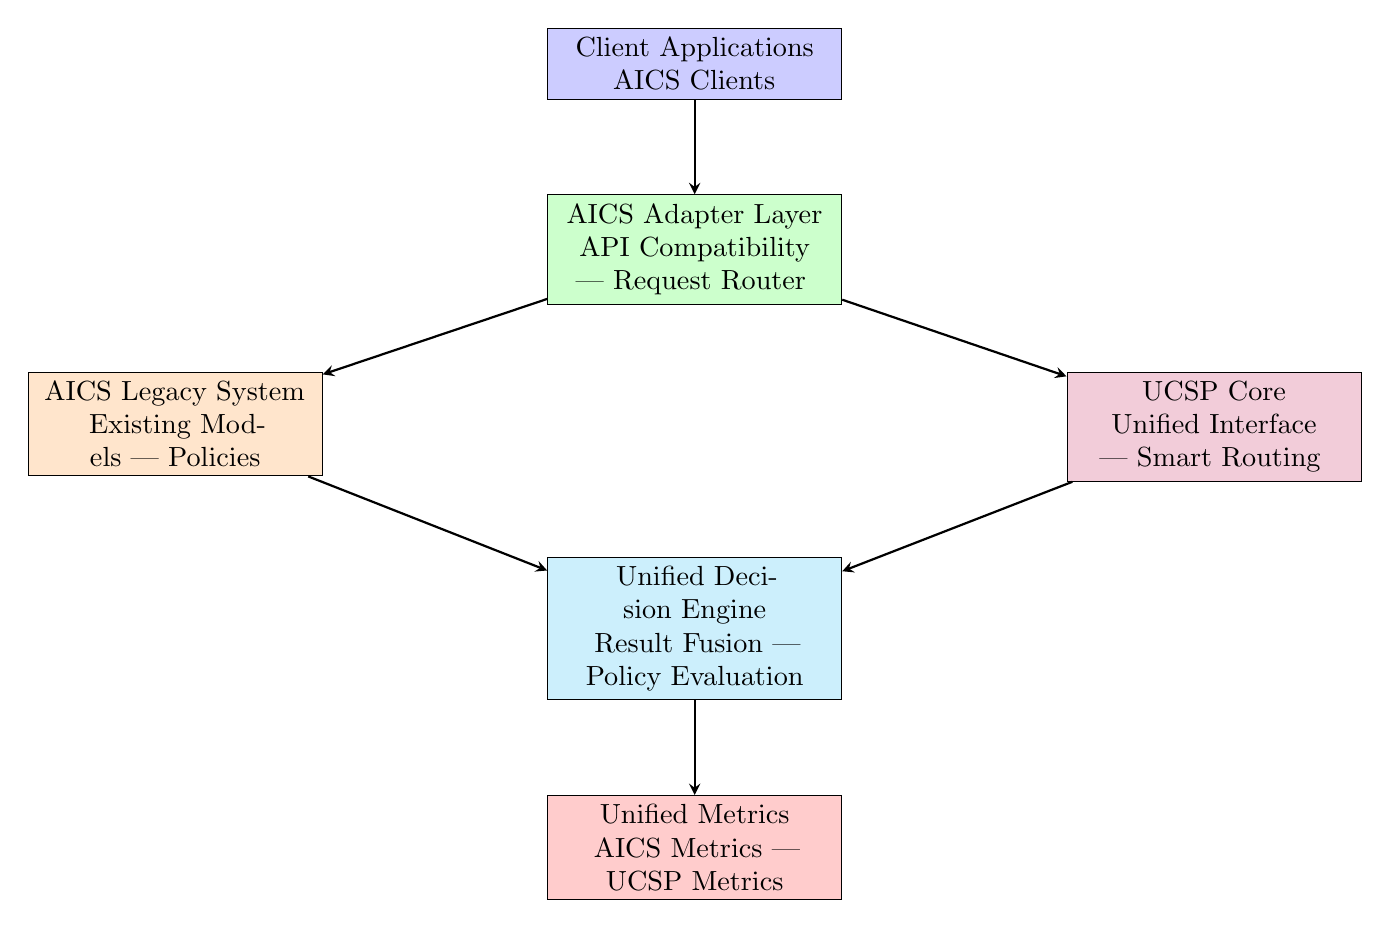
\begin{tikzpicture}[
    node distance=1.2cm,
    box/.style={rectangle, draw, text width=3.5cm, text centered, minimum height=0.8cm},
    arrow/.style={->, >=stealth, thick}
]
    \node[box, fill=blue!20] (client) {Client Applications\\AICS Clients};
    \node[box, fill=green!20, below=of client] (adapter) {AICS Adapter Layer\\API Compatibility | Request Router};
    \node[box, fill=orange!20, below left=of adapter, xshift=-2cm] (aics) {AICS Legacy System\\Existing Models | Policies};
    \node[box, fill=purple!20, below right=of adapter, xshift=2cm] (ucsp) {UCSP Core\\Unified Interface | Smart Routing};
    \node[box, fill=cyan!20, below=of adapter, yshift=-2cm] (unified) {Unified Decision Engine\\Result Fusion | Policy Evaluation};
    \node[box, fill=red!20, below=of unified] (metrics) {Unified Metrics\\AICS Metrics | UCSP Metrics};
    
    \draw[arrow] (client) -- (adapter);
    \draw[arrow] (adapter) -- (aics);
    \draw[arrow] (adapter) -- (ucsp);
    \draw[arrow] (aics) -- (unified);
    \draw[arrow] (ucsp) -- (unified);
    \draw[arrow] (unified) -- (metrics);
\end{tikzpicture}
\caption{AICS集成UCSP架构}
\label{fig:aics-integration}
\end{figure}

\subsection{适配器层设计}

\textbf{AICS适配器(AICS Adapter)职责:}
\begin{itemize}
    \item API兼容:将AICS原有API调用转换为UCSP统一接口
    \item 请求路由:根据配置将请求路由到AICS或UCSP
    \item 结果转换:将UCSP结果转换为AICS格式,保持兼容性
    \item 双路验证:在迁移阶段同时调用AICS和UCSP,对比结果
\end{itemize}

\textbf{适配器配置结构:}

\begin{lstlisting}[style=pseudocode, caption=AICS适配器配置]
STRUCT AICSAdapterConfig:
    adapter_id: UINT64
    aics_endpoint: STRING              // AICS服务端点
    ucsp_endpoint: STRING              // UCSP服务端点
    routing_mode: ENUM                 // 路由模式
        VALUES: [LEGACY_ONLY, UCSP_ONLY, DUAL_PATH, GRAYSCALE]
    grayscale_ratio: FLOAT          // 灰度比例(当模式为GRAYSCALE时)
    enable_dual_verification: BOOLEAN  // 是否启用双路验证
    result_fusion_strategy: ENUM   // 结果融合策略
        VALUES: [AICS_PRIORITY, UCSP_PRIORITY, CONSENSUS, CONFIDENCE_BASED]
    compatibility_mode: BOOLEAN     // 兼容模式:保持AICS响应格式
END STRUCT
\end{lstlisting}

\textbf{适配器路由算法:}

\begin{algorithm}[H]
\caption{AICS适配器路由算法}
\begin{algorithmic}[1]
\STATE 输入:AICS请求 $aics\_request$,适配器配置 $config$
\STATE 输出:安全检查响应 $response$
\STATE
\STATE // 根据路由模式决定处理路径
\IF{$config.routing\_mode == LEGACY\_ONLY$}
    \STATE $result \leftarrow CallAICS(aics\_request, config.aics\_endpoint)$
    \RETURN $ConvertToAICSFormat(result)$
\ELSIF{$config.routing\_mode == UCSP\_ONLY$}
    \STATE $ucsp\_request \leftarrow ConvertToUCSPFormat(aics\_request)$
    \STATE $result \leftarrow CallUCSP(ucsp\_request, config.ucsp\_endpoint)$
    \RETURN $ConvertToAICSFormat(result)$
\ELSIF{$config.routing\_mode == DUAL\_PATH$}
    \STATE // 双路验证:同时调用AICS和UCSP
    \STATE $aics\_result \leftarrow CallAICS(aics\_request, config.aics\_endpoint)$
    \STATE $ucsp\_request \leftarrow ConvertToUCSPFormat(aics\_request)$
    \STATE $ucsp\_result \leftarrow CallUCSP(ucsp\_request, config.ucsp\_endpoint)$
    \STATE $final\_result \leftarrow FuseResults(aics\_result, ucsp\_result, config)$
    \STATE $RecordComparison(aics\_result, ucsp\_result)$
    \RETURN $ConvertToAICSFormat(final\_result)$
\ELSIF{$config.routing\_mode == GRAYSCALE$}
    \STATE // 灰度发布:基于用户ID路由
    \STATE $user\_id \leftarrow ExtractUserID(aics\_request)$
    \STATE $hash \leftarrow MurmurHash3(user\_id \oplus config.adapter\_id)$
    \STATE $bucket \leftarrow hash \bmod 10000$
    \STATE $threshold \leftarrow config.grayscale\_ratio \times 10000$
    \IF{$bucket < threshold$}
        \STATE // 走UCSP路径
        \STATE $ucsp\_request \leftarrow ConvertToUCSPFormat(aics\_request)$
        \STATE $result \leftarrow CallUCSP(ucsp\_request, config.ucsp\_endpoint)$
        \IF{$config.enable\_dual\_verification$}
            \STATE $aics\_result \leftarrow CallAICS(aics\_request, config.aics\_endpoint)$
            \STATE $RecordComparison(aics\_result, result)$
        \ENDIF
    \ELSE
        \STATE // 走AICS路径
        \STATE $result \leftarrow CallAICS(aics\_request, config.aics\_endpoint)$
    \ENDIF
    \RETURN $ConvertToAICSFormat(result)$
\ENDIF
\end{algorithmic}
\end{algorithm}

\subsection{结果融合策略}

\textbf{结果融合算法:}

\begin{algorithm}[H]
\caption{AICS与UCSP结果融合算法}
\begin{algorithmic}[1]
\STATE 输入:AICS结果 $aics\_result$,UCSP结果 $ucsp\_result$,融合策略 $strategy$
\STATE 输出:融合后的结果 $fused\_result$
\STATE
\IF{$strategy == AICS\_PRIORITY$}
    \STATE // AICS优先:仅在AICS不确定时使用UCSP结果
    \IF{$aics\_result.confidence < UNCERTAIN\_THRESHOLD$}
        \RETURN $ucsp\_result$
    \ELSE
        \RETURN $aics\_result$
    \ENDIF
\ELSIF{$strategy == UCSP\_PRIORITY$}
    \STATE // UCSP优先:仅在UCSP不确定时使用AICS结果
    \IF{$ucsp\_result.confidence < UNCERTAIN\_THRESHOLD$}
        \RETURN $aics\_result$
    \ELSE
        \RETURN $ucsp\_result$
    \ENDIF
\ELSIF{$strategy == CONSENSUS$}
    \STATE // 共识策略:两者都拦截或都放行时采用,否则采用更严格的结果
    \IF{$aics\_result.blocked == ucsp\_result.blocked$}
        \RETURN $aics\_result$  \COMMENT{一致时采用AICS结果保持兼容}
    \ELSE
        \STATE // 不一致时,采用更严格的结果(拦截优先)
        \IF{$aics\_result.blocked$}
            \RETURN $aics\_result$
        \ELSE
            \RETURN $ucsp\_result$
        \ENDIF
    \ENDIF
\ELSIF{$strategy == CONFIDENCE\_BASED$}
    \STATE // 置信度策略:选择置信度更高的结果
    \IF{$aics\_result.confidence > ucsp\_result.confidence$}
        \RETURN $aics\_result$
    \ELSE
        \RETURN $ucsp\_result$
    \ENDIF
\ENDIF
\end{algorithmic}
\end{algorithm}

\subsection{数据迁移方案}

\textbf{迁移策略:}

\begin{algorithm}[H]
\caption{AICS数据迁移流程}
\begin{algorithmic}[1]
\STATE 输入:AICS数据源 $aics\_data$
\STATE
\STATE // 阶段1:数据导出
\STATE $exported\_data \leftarrow ExportAICSData(aics\_data)$
\STATE $ValidateDataFormat(exported\_data)$
\STATE
\STATE // 阶段2:数据转换
\STATE $converted\_data \leftarrow ConvertToUCSPFormat(exported\_data)$
\STATE $ValidateUCSPFormat(converted\_data)$
\STATE
\STATE // 阶段3:数据导入(分批进行)
\STATE $batches \leftarrow SplitIntoBatches(converted\_data, BATCH\_SIZE)$
\FOR{$batch$ IN $batches$}
    \STATE $ImportToUCSP(batch)$
    \STATE $VerifyImport(batch)$
    \IF{NOT $VerifyImport(batch)$}
        \STATE $RollbackBatch(batch)$
        \STATE $LogError("Batch import failed", batch)$
    \ENDIF
\ENDFOR
\STATE
\STATE // 阶段4:数据一致性验证
\STATE $VerifyDataConsistency(aics\_data, ucsp\_data)$
\STATE
\STATE // 阶段5:切换流量
\STATE $SwitchTrafficToUCSP()$
\end{algorithmic}
\end{algorithm}

\textbf{配置迁移:}

\begin{algorithm}[H]
\caption{AICS配置迁移算法}
\begin{algorithmic}[1]
\STATE 输入:AICS配置 $aics\_config$
\STATE 输出:UCSP配置 $ucsp\_config$
\STATE
\STATE // 模型配置迁移
\STATE $ucsp\_config.fast\_model \leftarrow MapAICSModel(aics\_config.primary\_model)$
\STATE $ucsp\_config.deep\_model \leftarrow MapAICSModel(aics\_config.fallback\_model)$
\STATE
\STATE // 策略配置迁移
\STATE $ucsp\_config.policy \leftarrow ConvertAICSPolicy(aics\_config.policy)$
\STATE
\STATE // 阈值配置迁移
\STATE $ucsp\_config.block\_threshold \leftarrow aics\_config.block\_threshold$
\STATE $ucsp\_config.warn\_threshold \leftarrow aics\_config.warn\_threshold$
\STATE
\STATE // 验证配置有效性
\STATE $ValidateUCSPConfig(ucsp\_config)$
\RETURN $ucsp\_config$
\end{algorithmic}
\end{algorithm}

\subsection{渐进式迁移方案}

\textbf{迁移阶段规划:}

\begin{enumerate}
    \item \textbf{阶段1:影子模式(Shadow Mode)}
    \begin{itemize}
        \item 所有请求走AICS,同时异步调用UCSP
        \item 对比AICS和UCSP结果,收集差异数据
        \item 评估UCSP性能和准确性
        \item 持续时间:2-4周
    \end{itemize}
    
    \item \textbf{阶段2:小流量验证(1\%-5\%)}
    \begin{itemize}
        \item 1\%流量走UCSP,99\%走AICS
        \item 双路验证,确保结果一致性
        \item 监控UCSP稳定性指标
        \item 持续时间:2-3周
    \end{itemize}
    
    \item \textbf{阶段3:逐步增加(5\%-50\%)}
    \begin{itemize}
        \item 每周增加5-10\%流量
        \item 持续监控和调整
        \item 处理发现的问题
        \item 持续时间:6-8周
    \end{itemize}
    
    \item \textbf{阶段4:全量切换(50\%-100\%)}
    \begin{itemize}
        \item 逐步增加到100\%
        \item AICS作为兜底备用
        \item 最终完全切换到UCSP
        \item 持续时间:4-6周
    \end{itemize}
\end{enumerate}

\textbf{迁移监控指标:}

\begin{algorithm}[H]
\caption{迁移监控算法}
\begin{algorithmic}[1]
\STATE 输入:迁移配置 $migration\_config$
\STATE
\STATE // 实时监控指标
\STATE $metrics \leftarrow GetMigrationMetrics(migration\_config)$
\STATE
\STATE // 一致性指标
\STATE $agreement\_rate \leftarrow CalculateAgreementRate(metrics.aics\_results, metrics.ucsp\_results)$
\STATE
\STATE // 性能指标
\STATE $ucsp\_latency \leftarrow CalculateAverageLatency(metrics.ucsp\_requests)$
\STATE $aics\_latency \leftarrow CalculateAverageLatency(metrics.aics\_requests)$
\STATE
\STATE // 准确性指标
\STATE $ucsp\_accuracy \leftarrow CalculateAccuracy(metrics.ucsp\_results, metrics.ground\_truth)$
\STATE $aics\_accuracy \leftarrow CalculateAccuracy(metrics.aics\_results, metrics.ground\_truth)$
\STATE
\STATE // 决策:是否继续迁移
\IF{$agreement\_rate > MIN\_AGREEMENT\_RATE$ AND 
    $ucsp\_latency < LATENCY\_THRESHOLD$ AND
    $ucsp\_accuracy \geq aics\_accuracy$}
    \STATE $IncreaseMigrationRatio(migration\_config)$
\ELSE
    \STATE $PauseMigration(migration\_config)$
    \STATE $TriggerAlert("Migration paused due to metrics degradation")$
\ENDIF
\end{algorithmic}
\end{algorithm}

\subsection{统一监控与可观测性}

\textbf{统一指标聚合:}

\begin{algorithm}[H]
\caption{统一指标聚合算法}
\begin{algorithmic}[1]
\STATE 输入:AICS指标 $aics\_metrics$,UCSP指标 $ucsp\_metrics$
\STATE 输出:统一指标 $unified\_metrics$
\STATE
\STATE // 聚合请求量
\STATE $unified\_metrics.total\_requests \leftarrow aics\_metrics.requests + ucsp\_metrics.requests$
\STATE
\STATE // 聚合拦截量
\STATE $unified\_metrics.total\_blocked \leftarrow aics\_metrics.blocked + ucsp\_metrics.blocked$
\STATE
\STATE // 计算平均延迟(加权平均)
\STATE $aics\_weight \leftarrow aics\_metrics.requests / unified\_metrics.total\_requests$
\STATE $ucsp\_weight \leftarrow ucsp\_metrics.requests / unified\_metrics.total\_requests$
\STATE $unified\_metrics.avg\_latency \leftarrow aics\_weight \times aics\_metrics.avg\_latency + ucsp\_weight \times ucsp\_metrics.avg\_latency$
\STATE
\STATE // 聚合错误率
\STATE $unified\_metrics.error\_rate \leftarrow (aics\_metrics.errors + ucsp\_metrics.errors) / unified\_metrics.total\_requests$
\STATE
\STATE // 计算迁移进度
\STATE $unified\_metrics.migration\_progress \leftarrow ucsp\_metrics.requests / unified\_metrics.total\_requests$
\STATE
\RETURN $unified\_metrics$
\end{algorithmic}
\end{algorithm}

\section{性能优化}

\subsection{缓存策略}

\begin{algorithm}[H]
\caption{带缓存的内容检查}
\begin{algorithmic}[1]
\STATE 输入:文本 $text$,用户ID $user\_id$
\STATE 输出:安全检查结果 $result$
\STATE
\STATE $cache\_key \leftarrow HashText(text)$
\STATE $cached\_result \leftarrow Cache.Get(cache\_key)$
\IF{$cached\_result \neq NULL$}
    \RETURN $cached\_result$
\ENDIF
\STATE
\STATE $result \leftarrow CheckContent(text, user\_id)$
\IF{$result.confidence > 0.90$}
    \STATE $Cache.Set(cache\_key, result, TTL=3600)$  \COMMENT{1小时TTL}
\ENDIF
\RETURN $result$
\end{algorithmic}
\end{algorithm}

\subsection{批量处理优化}

\begin{algorithm}[H]
\caption{批量检查优化}
\begin{algorithmic}[1]
\STATE 输入:请求列表 $requests[]$
\STATE 输出:结果列表 $results[]$
\STATE
\STATE $fast\_batch \leftarrow []$
\STATE $deep\_batch \leftarrow []$
\STATE
\FOR{$request$ IN $requests$}
    \STATE $quick\_check \leftarrow QuickPreCheck(request.text)$
    \IF{$quick\_check.confidence > 0.95$}
        \STATE $fast\_batch.APPEND(request)$
    \ELSE
        \STATE $deep\_batch.APPEND(request)$
    \ENDIF
\ENDFOR
\STATE
\STATE $fast\_results \leftarrow PARALLEL FastModel.BatchInference(fast\_batch)$
\STATE $deep\_results \leftarrow PARALLEL DeepModel.BatchInference(deep\_batch)$
\RETURN $MERGE(fast\_results, deep\_results)$
\end{algorithmic}
\end{algorithm}

\section{监控与可观测性}

\subsection{实时指标监控}

\begin{algorithm}[H]
\caption{指标更新算法}
\begin{algorithmic}[1]
\STATE 输入:安全检查结果 $result$,处理时间 $processing\_time$
\STATE
\STATE ATOMIC INCREMENT $metrics.total\_requests$
\IF{$result.blocked$}
    \STATE ATOMIC INCREMENT $metrics.blocked\_count$
\ENDIF
\STATE
\STATE UPDATE $latency\_histogram(processing\_time)$
\STATE $metrics.avg\_latency\_ms \leftarrow CalculateAverage(latency\_histogram)$
\STATE $metrics.p95\_latency\_ms \leftarrow CalculatePercentile(latency\_histogram, 0.95)$
\STATE $metrics.p99\_latency\_ms \leftarrow CalculatePercentile(latency\_histogram, 0.99)$
\STATE
\IF{$result.model\_version == FAST\_MODEL\_VERSION$}
    \STATE INCREMENT $fast\_model\_hits$
\ELSE
    \STATE INCREMENT $deep\_model\_hits$
\ENDIF
\STATE
\STATE $metrics.fast\_model\_hit\_rate \leftarrow fast\_model\_hits / metrics.total\_requests$
\STATE $metrics.deep\_model\_hit\_rate \leftarrow deep\_model\_hits / metrics.total\_requests$
\end{algorithmic}
\end{algorithm}

\subsection{告警机制}

\begin{algorithm}[H]
\caption{告警检查算法}
\begin{algorithmic}[1]
\STATE 输入:系统指标 $metrics$
\STATE
\IF{$metrics.p95\_latency\_ms > LATENCY\_THRESHOLD$}
    \STATE $TriggerAlert("High latency detected", metrics.p95\_latency\_ms)$
\ENDIF
\STATE
\STATE $false\_positive\_rate \leftarrow metrics.false\_positive\_count / metrics.total\_requests$
\IF{$false\_positive\_rate > FALSE\_POSITIVE\_THRESHOLD$}
    \STATE $TriggerAlert("High false positive rate", false\_positive\_rate)$
\ENDIF
\STATE
\STATE $false\_negative\_rate \leftarrow metrics.false\_negative\_count / metrics.total\_requests$
\IF{$false\_negative\_rate > FALSE\_NEGATIVE\_THRESHOLD$}
    \STATE $TriggerAlert("High false negative rate", false\_negative\_rate)$
\ENDIF
\STATE
\IF{$metrics.fast\_model\_hit\_rate < MIN\_HIT\_RATE$}
    \STATE $TriggerAlert("Fast model performance degraded")$
\ENDIF
\end{algorithmic}
\end{algorithm}

\section{实施路线图}

\subsection{阶段一:核心功能实现(1-2个月)}

\textbf{目标:}实现统一接口和智能路由

\textbf{任务:}
\begin{enumerate}
    \item 实现 Safety Gateway
    \item 部署 Fast Model 和 Deep Model
    \item 实现统一接口 CheckContent
    \item 实现智能路由算法
\end{enumerate}

\textbf{验收标准:}
\begin{itemize}
    \item 90\% 请求在快速模型完成
    \item 平均延迟 < 50ms
    \item 接口可用性 > 99.9\%
\end{itemize}

\subsection{阶段二:灰度发布框架(2-3个月)}

\textbf{目标:}实现灰度发布,逐步接管Vendor流量

\textbf{任务:}
\begin{enumerate}
    \item 实现灰度发布路由算法
    \item 实现双路验证机制
    \item 实现自动流量调整
    \item 实现成本控制算法
    \item 实现稳定性检查与快速回滚
\end{enumerate}

\textbf{灰度发布计划:}
\begin{itemize}
    \item \textbf{第1周:} 1\% 流量验证,双路对比,确保稳定性
    \item \textbf{第2-3周:} 5\% 流量验证,持续监控指标
    \item \textbf{第4-5周:} 10\% 流量,验证成本控制
    \item \textbf{第6-7周:} 20\% 流量,验证系统负载
    \item \textbf{第8-9周:} 50\% 流量,验证大规模场景
    \item \textbf{第10-11周:} 80\% 流量,接近全量
    \item \textbf{第12周:} 100\% 流量,完全接管
\end{itemize}

\textbf{验收标准:}
\begin{itemize}
    \item 支持1\%-100\%流量比例动态调整
    \item 稳定性指标(误杀率、漏判率)< 阈值
    \item 成本控制在预算范围内
    \item 支持秒级回滚
    \item 与Vendor结果一致性 > 95\%
\end{itemize}

\subsection{阶段三:A/B 测试框架(3-4个月)}

\textbf{目标:}实现确定性 A/B 测试

\textbf{任务:}
\begin{enumerate}
    \item 实现确定性路由算法
    \item 实现指标收集系统
    \item 实现统计显著性检测
    \item 实现实验管理界面
\end{enumerate}

\textbf{验收标准:}
\begin{itemize}
    \item 支持多实验并行
    \item 指标实时更新
    \item 自动决策支持
\end{itemize}

\subsection{阶段四:策略管理系统(4-5个月)}

\textbf{目标:}实现代码驱动的策略管理

\textbf{任务:}
\begin{enumerate}
    \item 实现策略定义框架
    \item 实现策略版本管理
    \item 实现策略测试框架
    \item 实现策略部署流程
\end{enumerate}

\textbf{验收标准:}
\begin{itemize}
    \item 策略变更可追溯
    \item 策略可单元测试
    \item 支持策略回滚
\end{itemize}

\section{总结}

本设计文档阐述了一个统一的内容安全平台架构,通过统一接口设计、智能路由、确定性A/B测试和代码驱动的策略管理等核心技术,实现了高性能、高可维护性的内容安全检查系统。该架构具有以下优势:

\begin{enumerate}
    \item \textbf{高性能:} 90\% 请求在 20ms 内完成,整体平均延迟 < 35ms
    \item \textbf{高可维护性:} 统一接口设计,代码量减少 60\%
    \item \textbf{科学验证:} 确定性 A/B 测试框架,支持策略科学验证
    \item \textbf{可追溯性:} 策略版本管理,所有变更可追溯
    \item \textbf{可扩展性:} 模块化设计,易于扩展新功能
    \item \textbf{平滑迁移:} 灰度发布策略,支持从Vendor逐步切换到自研系统
    \item \textbf{向后兼容:} AICS集成设计,实现现有系统平滑迁移,保持业务连续性
\end{enumerate}

该架构为构建企业级内容安全平台提供了坚实的技术基础,同时支持从现有系统(如AICS)平滑迁移,降低了系统升级的风险和成本。

\end{document}
